Alex Iverson

2015-01-19

Pruning and Redesigning

\begin{tabular}{|p{5cm}|p{5cm}|}
 \hline
 We removed the damaged components from the robot and the things that need to be updated. &
 The damaged guide tube has been removed. The intake has been removed and is in the process of being replaced.
 \\
 \hline
 Deflector improvements. &
 I put together a set of modifications to the deflector that should allow it to handle large balls reliably and score more accurately.
 \\
 \hline
\end{tabular}

I recomputed the angles and lengths of the deflector so that it provides enough room for a large ball to fit through easily and so that it lines up with the mouth of a goal being handled by our robot.
The geometric changes were fairly simple, but they did necessitate a full rebuild of the deflector. Communicating what needed to be done for the deflector proved more time consuming than it should have been.
\begin{center}
 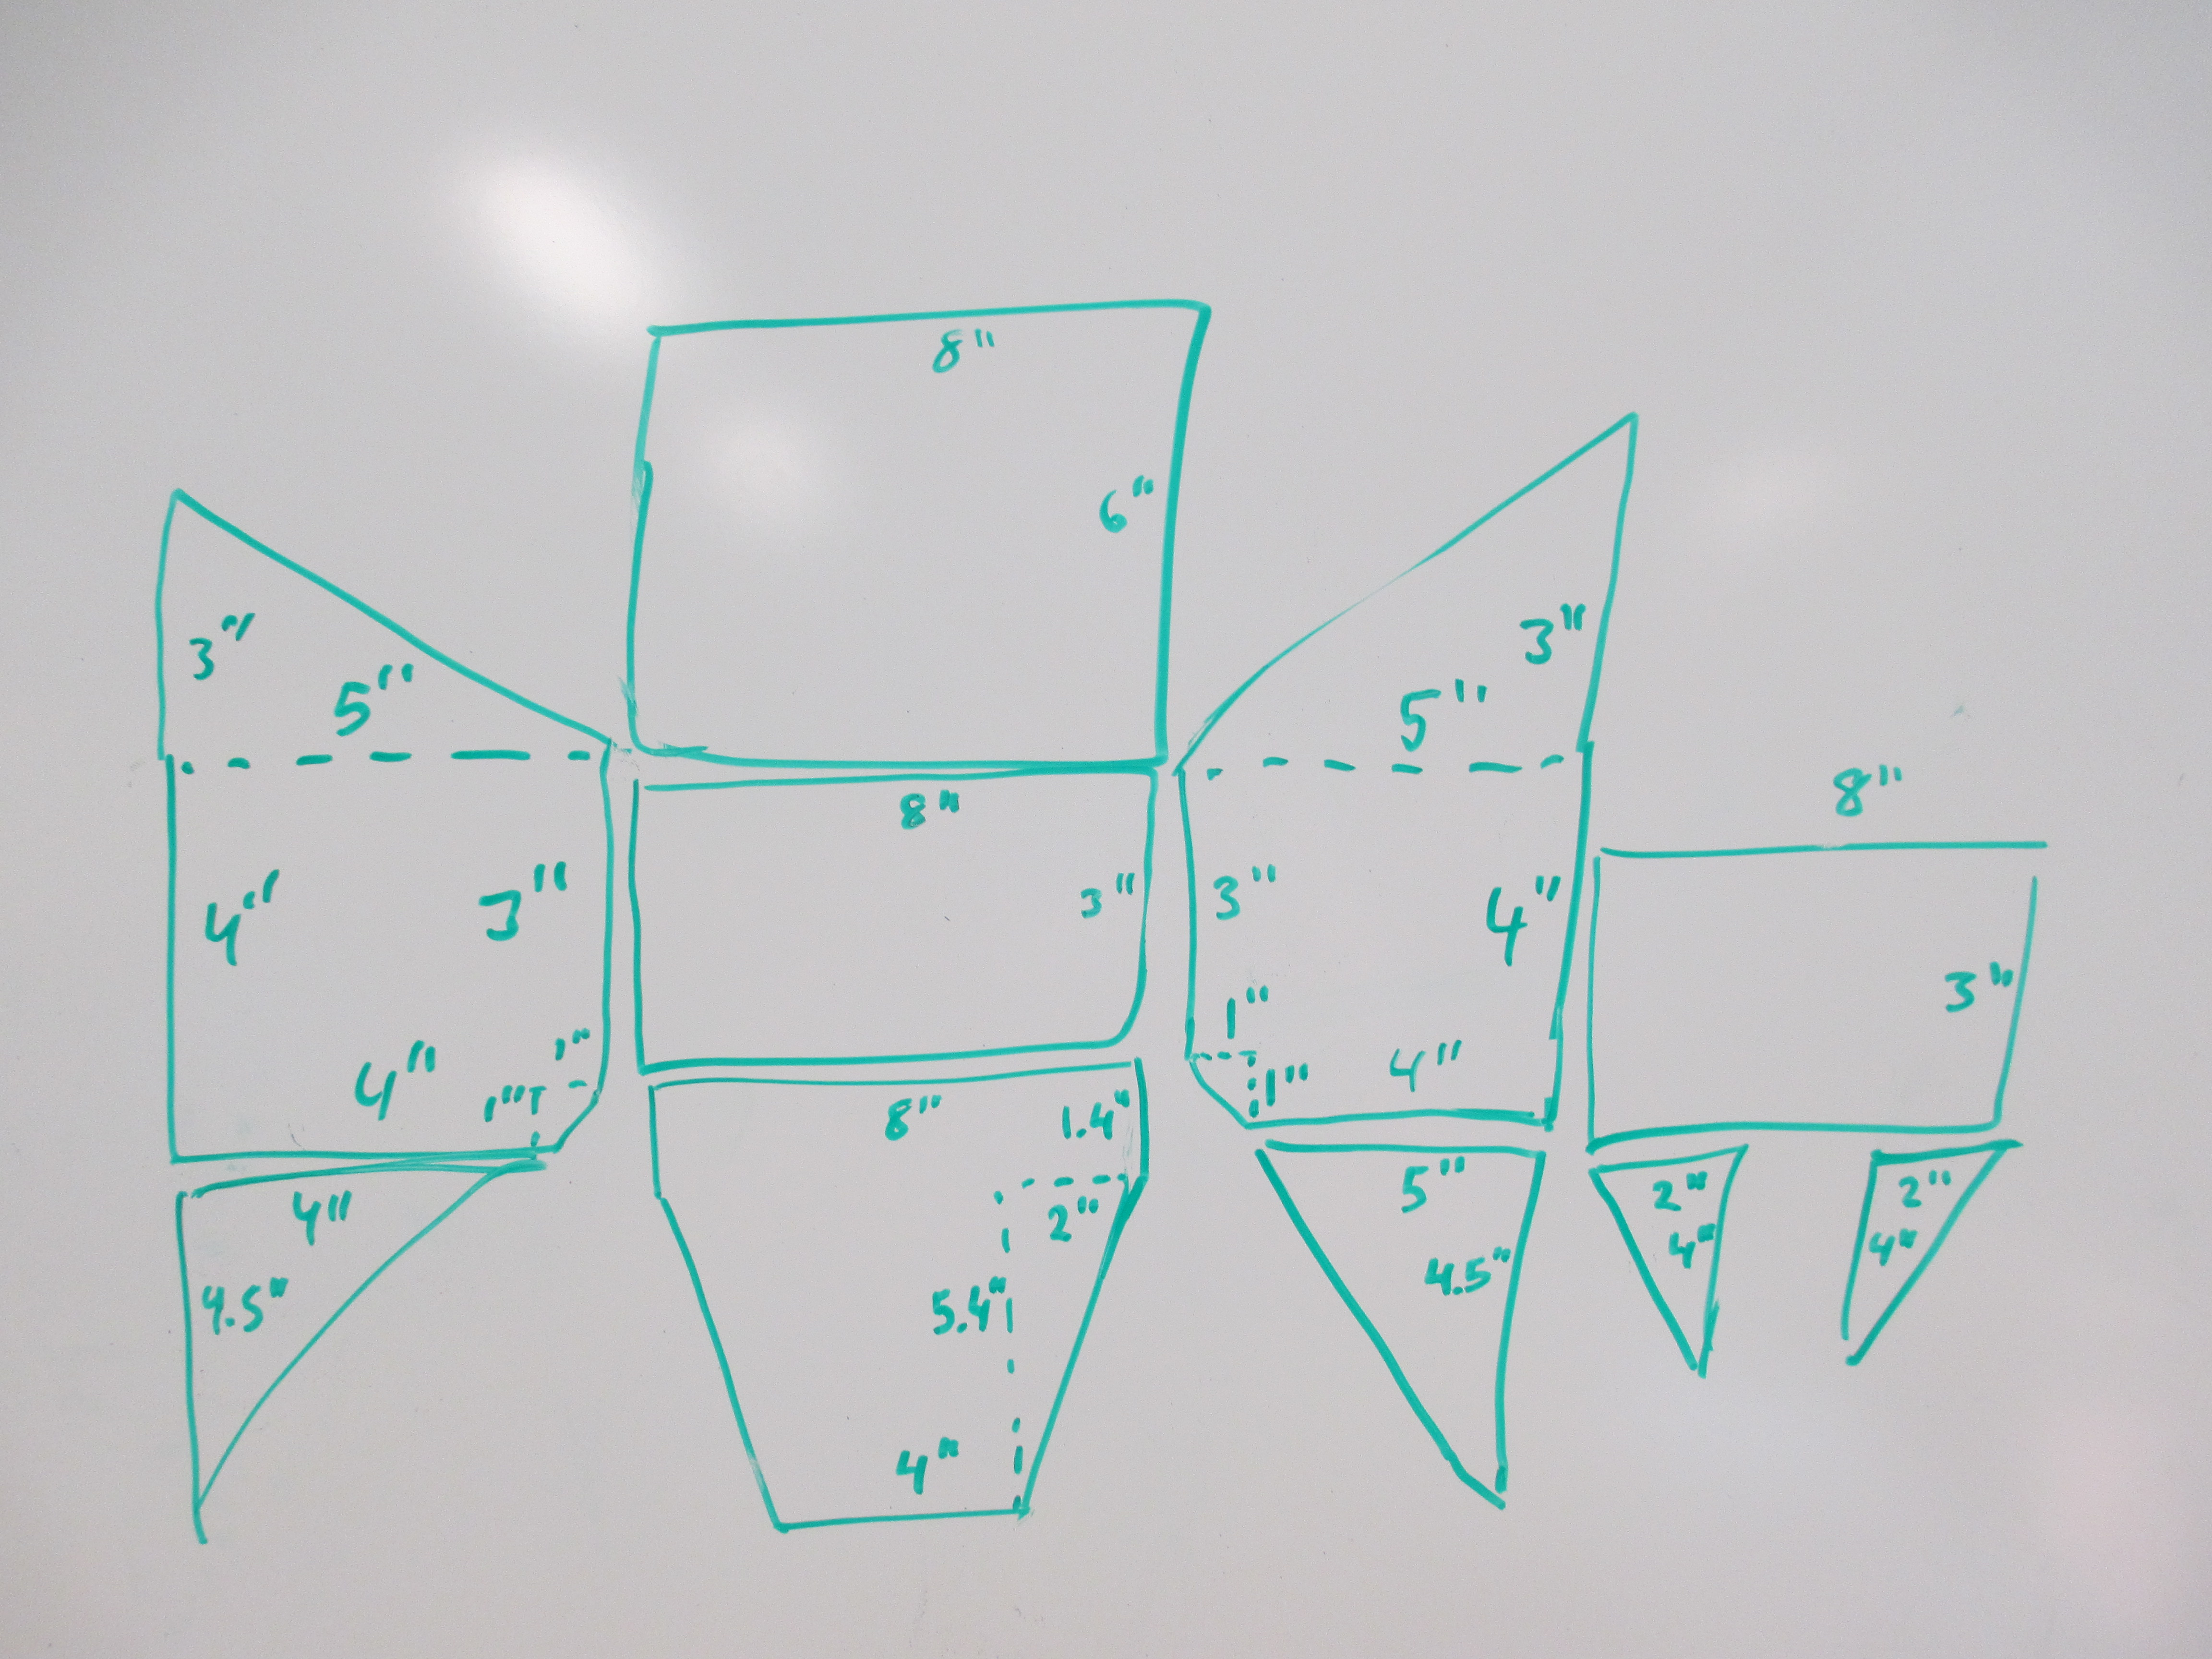
\includegraphics[width=10cm]{./Entries/Images/deflectorDiagramFinal.JPG}
\end{center}
